%%%% This is the file with a chapter body from the SPbPU-BCI template  %%%%
%%%%
   \renewcommand{\chapterEnTitle}{Eleventh chapter title} 
%% Input the English title here (only once!). 
%% Please, type in titles small letters except for the first letter in the first word and names of persons etc.
%% Заполнять по правилам русского языка, не оформляя каждое слово с прописной буквы (заполняется только один раз). 
%%
%%%%
   \renewcommand{\chapterRuTitle}{Название одиннадцатой главы}          
%% For non-Russian authors the text can be submitted as-is and translated by editors.
%% Введите заголовок по-русски  (только один раз здесь!).
%%
%%%%
   \setcounter{mychapternumber}{11} 
%% Input chapter number in case of chapter acceptance. 
%% введите номер главы в случае принятия главы. 
%% 
%%%% 
   \hyphenation{Diag-nos-tic-Tests-Sca-ling-And-In-fer-ring длинное-название-возможно-например-на-немецком long-title-possible-for example-in-German} 
%% для редких и/или длинных названий, например, алгоритмов необходимо задать правила переноса на нову строчку по слогам


%%%% START OF EPIGRAPH AND TITLE (PLEASE, DO NOT MODIFY) %%%%
%%%% НАЧАЛО ЭПИГРАФА И НАЗВАНИЯ (НЕ ВНОСИТЬ ИЗМЕНЕНИЯ) %%%% 
{%
	\cleardoublepage
	\let\clearpage\relax
	\setcounter{chapter}{\value{mychapternumber}-1} 
	\setcounter{chapterDOI}{\value{mychapternumber}+2}
	\begin{flushleft}
	\smallA{\href{http://dx.doi.org/10.18720/SPBPU/2/id17-1_\thechapterDOI}{DOI 10.18720/SPBPU/2/id17-1\_\thechapterDOI}}
	\vspace{2\curtextsize}
	\end{flushleft}	
	\chapter{\chapterEnTitle} \label{chapt1}
	\addtocen{chapter}{\chapterEnTitle} 
	\addtocru{chapter}{\chapterRuTitle} 
}%
%%%% КОНЕЦ ЭПИГРАФА И НАЗВАНИЯ (НЕ ВНОСИТЬ ИЗМЕНЕНИЯ) %%%%
%%%% END OF EPIGRAPH AND TITLE (PLEASE, DO NOT MODIFY)  %%%% % keep unmodified

	
\smallA{\itshape%
%%%%
%%		
%%  Please, write the information in English
%%		
%%  Пожалуйта, заполните информацию на английском
%%		
	Name SecondName Surname of First Author, title of the position, organization, a address, %
	\mailtoMLABSEDauthor{email@spbstu.ru}{Dear Author}{email@spbstu.ru}. 
	%{true email}{email body}{represented email}
	\par 
	Name SecondName Surname of Second Author, title of the position, organization, a address, %
	\mailtoMLABSEDauthor{email@spbstu.ru}{Dear Author}{email@spbstu.ru}. 
	%{true email}{email body}{represented email}
	\par
	{\normalfont \abstractnameENG.} The text of the abstract in english (at least 70 and at most 150 words).
	\par
	{\normalfont \keywordsENG.} Three-six comma separated keywords.
	\par
	{\normalfont \acknowledgementsENG.} Acknowledgements, information about supporting grants and funds. Can be omitted. 
%%		
	\delnewpagebeforech % keep unmodified, including the following blank lines

%%
%%

	\chapter*{\thechapter. \chapterRuTitle} % keep unmodified
	
%%%%
%%		
%%  Please, write the information in Russian. For non-Russian authors the text can be submitted as-is and translated by editors.
%%		
%%  Пожалуйта, заполните информацию на русском
%%	
	Имя Отчество Фамилия первого автора, должность, организация, адрес, \mailtoMLABSEDauthor{email@spbstu.ru}{Dear Author}{email@spbstu.ru}. %{true email}{email body}{represented email}
	\par
	Имя Отчество Фамилия второго автора, должность, организация, адрес, \mailtoMLABSEDauthor{email@spbstu.ru}{Dear Author}{email@spbstu.ru}. %{true email}{email body}{represented email}
	\par
	{\normalfont \abstractname.} Текст аннотации на русском (минимум 70 и максимум 150 слов).   
	\par
	{\normalfont \keywords.} 6-7 ключевых слов через запятую.
	\par
	{\normalfont \acknowledgements.} Благодарности, информация о поддерживающих грантах и фондах. При необходимости. 
}%

%%%%
%%	Bibliography	
%%		
	\begin{refsection}[ch_folder_AuthorsSurnames/ch_bib_AuthorsSurnames.bib] %please rename <<AuthorsSurnames>>
		
	\newrefcontext[labelprefix=\thechapter.] % keep unmodified

	
%%%%
%%		
%%  The following text can be written in English or in Russian. 
%%  For non-Russian authors the text of titles of sections in Russian can be submitted as-is and translated by editors. 
%%  
	
	\section*{Введение} \label{sect1_1}
	
	Текст введения.


	\section{Название подраздела} \label{sect1_2} %название по-русски
	\addtocru{section}{Название подраздела} %повторите название по-русски
	\addtocen{section}{Section title} % title in english 
	
	А вот так пишется нумерованая формула:
	\begin{equation}
	\label{eq:equation1_1}
	e = \lim_{n \to \infty} \left( 1+\frac{1}{n} \right) ^n
	\end{equation}


\input{../SPbPU-examples-for-templates/tex/fig-spbpu-new-bld-autumn}	


	
	\begin{table} [htbp]% Пример записи таблицы с номером, но без отображаемого наименования
		\centering
			\caption{Оконная функция}%
			\label{tbl:test1_1}%
			\begin{SingleSpace}
				\begin{tabular}{  |c | c | c | c| }
					\hline
					Оконная функция	& ${2N}$ & ${4N}$	& ${8N}$	\\ \hline
					Прямоугольное 	& 8,72 	 & 8,77		& 8,77		\\ %\hline
					Ханна		& 7,96 	 & 7,93		& 7,93		\\ %\hline
					Хэмминга	& 8,72 	 & 8,77		& 8,77		\\ %\hline
					Блэкмана	& 8,72 	 & 8,77		& 8,77		\\ \hline
				\end{tabular}%
			\end{SingleSpace}
	\end{table}
	
	
	
	
	\section{Название подраздела} \label{sect1_3} %название по-русски
	\addtocru{section}{Название подраздела} %повторите название по-русски
	\addtocen{section}{Section title} % title in english 
	
	
	
	Название подраздела (на английском section) выносится в Содержание с абзацным отступом по ширине (или отступом, равным длине нумерационной части с пробелом). В терминологии ГОСТов название главы является разделом (на английском chapter). Отступ перед и после текста подраздела: 2 строки.
	
	

	
	\subsection{Название параграфа} \label{sect1_3_1} %название по-русски
	\addtocru{subsection}{Название параграфа} %повторите название по-русски
	\addtocen{subsection}{Paragraph title} % title in english 
	
	
	Название параграфа (на английском subsection)  выносится в Содержание с двумя абзацными отступами по ширине. Отступ перед и после текста: 1 строка. 
	
	
		
	\subsubsection{Название подпараграфа} \label{sect1_3_1_1} %название по-русски
	\addtocru{subsubsection}{Название подпараграфа} %повторите название по-русски
	\addtocen{subsubsection}{Subparagraph title} % title in english 
	
	
	
	
	Название подпараграфа (на английском subsubsection) переносится в содержание на усмотрение редакторов. Названия ненумеруемых подразделов {\itshape Введение, Выводы и Библиографический список} не выносятся в содержание.  Отступ перед и после текста: 1 строка.
	
	Когда есть необходимость ссылки в тексте документа на одно из перечислений и как правило {\itshape после параграфа или подпараграфа}, можно использовать нумерованные списки с иерархией:
	\begin{enumerate}
		\item первый пункт;
		\item второй пункт;
		\item по ГОСТ 2.105 первый уровень нумерации идёт буквами русского или латинского алфавитов ({\itshape для определенности выбираем английский алфавит}),
		а второй "--- цифрами: 
		\begin{enumerate}
			\item В нём лежит нумерованный список.
			\begin{enumerate}
				\item Ещё один нумерованный список;
				\item Третий уровень нумерации не нормирован ГОСТ 2.105 ({\itshape для определенности выбираем английский алфавит});
				\item Обращаем внимание на строчность букв в этом и следующем списке:
				\begin{itemize}
					\item Ещё один маркированный список.
				\end{itemize}    
			\end{enumerate}
		\end{enumerate}
		\item Четвёртый пункт.
	\end{enumerate}
	
	
	
	Оформление псевдокода необходимо осуществлять с помощью пакета \verb|algorithm2e|, следуя настройкам вывода, приведённым в примере (псевдокод оформляется как рисунок).
	
	
	\begin{algorithm} %[h]
		\SetKwFunction{algoDTestsFDSCALING}{} 
		\SetKwProg{myalg}{Algorithm}{}{} %write in 2nd agrument <<Algorithm>>, <<Procedure>> etc
		\nonl\myalg{\algoDTestsFDSCALING}{
			\KwInput{the many-valued context $\cont[M]\eqdef(G,M,W,J)$, the class membership $\epsilon: G\to K$} 
			\KwOutput{positive and negative binary contexts $\overbar{\cont[K]_+}\eqdef(\overbar{G_+},M,I_+)$, $\overbar{\cont[K]_-}\eqdef(\overbar{G_-},M,I_-)$ such that i-tests found in $\overbar{\cont[K]_+}$ are diagnostic tests in $\cont[M]$, and objects from $\overbar{\cont[K]_-}$ are counter-examples} %последние строки формируют начальное множество диагностических тестов
			\For {$\forall g_i,$ $g_j \in G$\label{FD-scaling-step-first}}{
				%(\tcp*[f]{possible inlined comment})
				\If{$i < j$ }{
					$\overbar{G} \leftarrow (g_i,g_j)$\;
				}
			}
			%		$M\leftarrow M\setminus k$\;
			\For {$\forall (g_i,g_j)\in \overbar{G}$}{
				%(\tcp*[f]{possible inlined comment})
				\If{$m(g_i) = m(g_j)$ }{ %на самом деле здесь цикл по всем компонентам вектора-строки
					$(g_i,g_j) I m$\; % or setI() function
				}
				\uIf{$\epsilon(g_i) = \epsilon(g_j)$ }{
					$\overbar{G_+} \leftarrow (g_i,g_j)$\;
				}
				\lElse{$\overbar{G_-} \leftarrow (g_i,g_j)$\label{FD-scaling-step-last}}	
			}		
			$I_+= I\cap (\overbar{G_+}\times M)$, $I_-= I\cap (\overbar{G_-}\times M)$\label{FD-scaling-step-newK}\; 
			\For {$\forall \overbar{g_+}\in \overbar{G_+}$, $\forall \overbar{g_-}\in \overbar{G_-}$ }{
				\If{$\overbar{g_+}\uA \subseteq \overbar{g_-}\uA$ }{
					$\overbar{G_+} \leftarrow \overbar{G_+} \setminus \overbar{g_+}$\;
				}
			}
			%		\Return \;
		}
		\caption{Псевдокод алгоритма \texttt{DiagnosticTestsScalingAndInferring}}\label{Alg-AlgoFDSCALING}
		% example of adding an item to Index
		% \index for accepted papers only
		\index[ru]{алгоритм! \texttt{название\_алгоритма}} 
		% key words <<алгоритм>> и <<algorithm>> keep unmodified
		\index[en]{algorithm! \texttt{algorighm\_title}}
		% authors can used the key word <<процедура>> (procedure) и т.п.
		%
		%
	    % another example:
		\index[ru]{алгоритм! \texttt{DiagnosticTestsScaling- AndInferring}}  %ключевые слова <<алгоритм>> и <<algorithm>> не менять
		\index[en]{algorithm! \texttt{DiagnosticTestsScaling- AndInferring}} 
	\end{algorithm} 
	
	% another example of adding an arbitrary keyword to Index
	% some useful keywords: theorem, proposition, lemma, equation etc
	% please, use short keywords (2-3 max)
	\index[ru]{длинное-название-возможное-например-на-немецком} % длинные названия первого уровня как правило запрещены
	\index[en]{long-title-possible-for-example-in-German} 
	
	Обратим внимание, что можно сослаться на строчку \ref{FD-scaling-step-first} псевдокода. При необходимости можно добавить подрисуночный комментарий.
	
	
	
	\section{Название подраздела} \label{sect1_4} %название по-русски
	\addtocru{section}{Название подраздела} %повторите название по-русски
	\addtocen{section}{Section title} % title in english  

	
Нумерованых формул может быть несколько:
\begin{equation}
\label{eq:equation1_2}
\lim_{n \to \infty} \sum_{k=1}^n \frac{1}{k^2} = \frac{\pi^2}{6}
\end{equation}

Впоследствии на формулы (\ref{eq:equation1_1}) и (\ref{eq:equation1_2}) можно ссылаться.

Сделать так, чтобы номер формулы стоял напротив средней строки, можно, используя окружение \verb|multlined| (пакет \verb|mathtools|) вместо \verb|multline| внутри окружения \verb|equation|. Вот так:
\begin{equation} % \tag{S} % tag - вписывает свой текст 
\label{eq:equation1_3}
\begin{multlined}
1+ 2+3+4+5+6+7+\dots + \\ 
+ 50+51+52+53+54+55+56+57 + \dots + \\ 
+ 96+97+98+99+100=5050 
\end{multlined}
\end{equation}

Используя команду \verb|\labelcref| из пакета \verb|cleveref|, можно
красиво ссылаться сразу на несколько формул
(\labelcref{eq:equation1_1,eq:equation1_3,eq:equation1_2}).


\begin{figure}[ht]
	\adjustbox{minipage=1.3em,valign=t}{\subcaption{}\label{sfig:testa}}%
	\begin{subfigure}[t]{\dimexpr.5\linewidth-1.3em\relax}
		\centering
		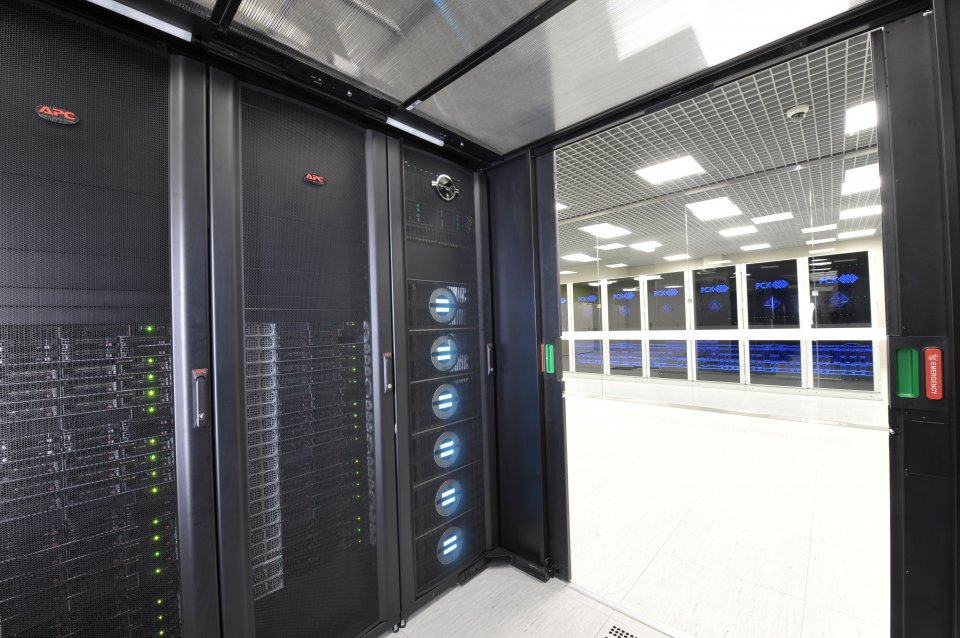
\includegraphics[width=.95\linewidth,valign=t]{spbpu_sc_system}
	\end{subfigure}
\hfill %выровнять по ширине
	\adjustbox{minipage=1.3em,valign=t}{\subcaption{}\label{sfig:testb}}%
	\begin{subfigure}[t]{\dimexpr.5\linewidth-1.3em\relax}
		\centering
		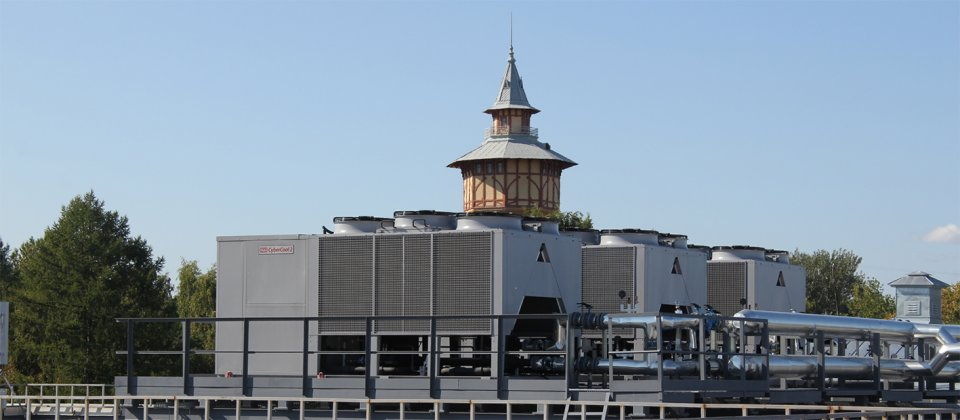
\includegraphics[width=.95\linewidth,valign=t]{spbpu_sc_refr}
	\end{subfigure}
\\[20pt]
	\adjustbox{minipage=1.3em,valign=t}{\subcaption{}\label{sfig:testc}}%
\begin{subfigure}[t]{\dimexpr.5\linewidth-1.3em\relax}
	\centering
	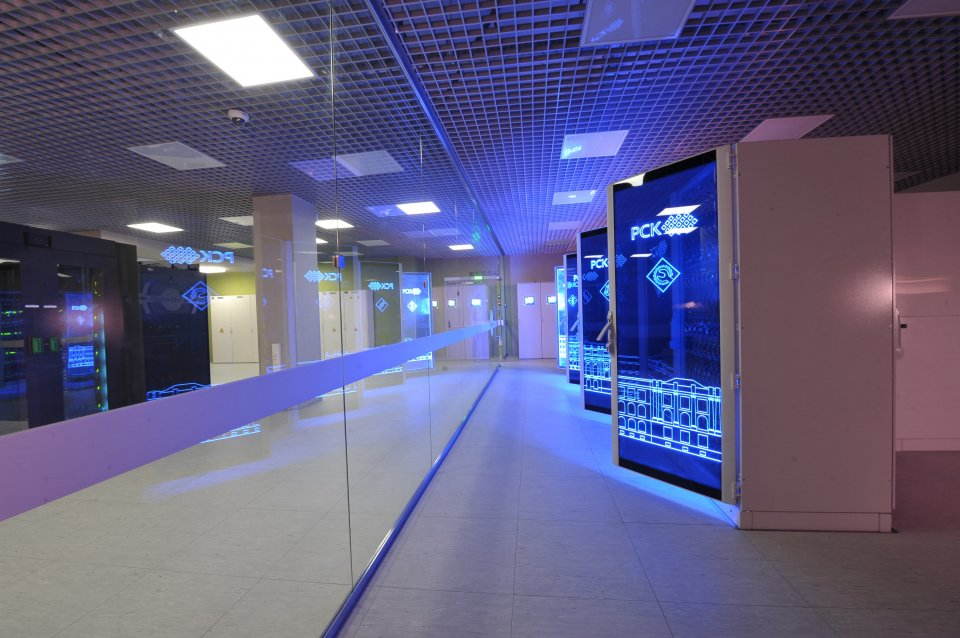
\includegraphics[width=.95\linewidth,valign=t]{spbpu_sc_hall}
\end{subfigure}%
\hfill %выровнять по ширине
\adjustbox{minipage=1.3em,valign=t}{\subcaption{}\label{sfig:testd}}%
\begin{subfigure}[t]{\dimexpr.5\linewidth-1.3em\relax}
	\centering
	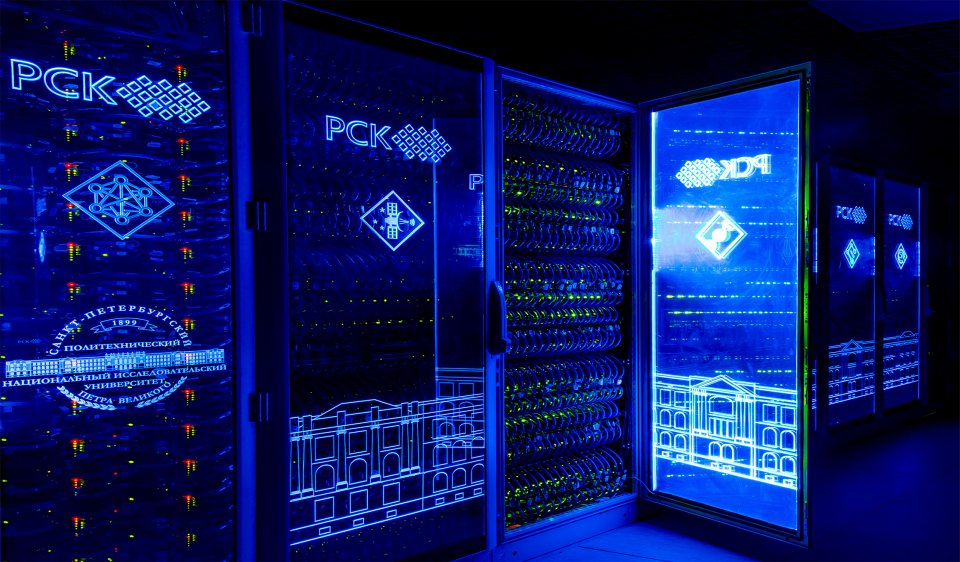
\includegraphics[width=.95\linewidth,valign=t]{spbpu_sc_box}
\end{subfigure}
\captionsetup{justification=centering} %центрировать
\caption{Фотографии суперкомпьютерного центра СПбПУ: {\itshape a} --- система хранения данных и узлы NUMA-вычислителя; {\itshape b} --- холодильные машины на крыше научно-исследовательского корпуса; {\itshape c} --- машинный зал; {\itshape d} --- элементы вычислительных устройств} 
\label{Fig:complexABCD}
\end{figure}

Далее можно ссылаться на рисунок \ref{sfig:testa}, \ref{sfig:testb}, \ref{sfig:testc}, \ref{sfig:testd} и рисунок \ref{Fig:complexABCD} в целом.

Пример длинной таблицы с записью продолжения по ГОСТ 2.105.
\begingroup
\centering
\smallA
\begin{longtable}[c]{|l|c|l|l|}
	\caption{Наименование таблицы средней длины}%
	\label{tbl:test5}% label всегда желательно идти после caption
	\\
	\hline
	%\multicolumn{4}{|c|}{\textbf{Файл puma\_namelist}}        \\ \hline
	Параметр & Умолч. & Тип & Описание\\ \hline
	\endfirsthead%
	%     \multicolumn{4}{|c|}{\small\slshape (продолжение)}        \\ \hline
	\captionsetup{format=tablenocaption,labelformat=continued}% должен стоять до самого caption
	\caption[]{}\\
	\hline
	Параметр & Умолч. & Тип & Описание\\ \hline
	\endhead
	\hline
	%     \multicolumn{4}{|r|}{\small\slshape продолжение следует}  \\
	%\hline
	\endfoot
	\hline
	\endlastfoot
	%     \multicolumn{4}{|l|}{\&INP}        \\ \hline 
	kick & 1 & int & 0: инициализация без шума ($p_s = const$) \\
	&   &     & 1: генерация белого шума                  \\
	&   &     & 2: генерация белого шума симметрично относительно \\
	& & & экватора    \\
	mars & 0 & int & 1: инициализация модели для планеты Марс     \\
	kick & 1 & int & 0: инициализация без шума ($p_s = const$) \\
	&   &     & 1: генерация белого шума                  \\
	&   &     & 2: генерация белого шума симметрично относительно \\
		& & & экватора    \\
	mars & 0 & int & 1: инициализация модели для планеты Марс     \\
	kick & 1 & int & 0: инициализация без шума ($p_s = const$) \\
	&   &     & 1: генерация белого шума                  \\
	&   &     & 2: генерация белого шума симметрично относительно \\
		& & & экватора    \\
	mars & 0 & int & 1: инициализация модели для планеты Марс     \\
	kick & 1 & int & 0: инициализация без шума ($p_s = const$) \\
	&   &     & 1: генерация белого шума                  \\
	&   &     & 2: генерация белого шума симметрично относительно \\
		& & & экватора    \\
	mars & 0 & int & 1: инициализация модели для планеты Марс     \\
	kick & 1 & int & 0: инициализация без шума ($p_s = const$) \\
	&   &     & 1: генерация белого шума                  \\
	&   &     & 2: генерация белого шума симметрично относительно \\
		& & & экватора    \\
	mars & 0 & int & 1: инициализация модели для планеты Марс     \\
	kick & 1 & int & 0: инициализация без шума ($p_s = const$) \\
	&   &     & 1: генерация белого шума                  \\
	&   &     & 2: генерация белого шума симметрично относительно \\
		& & & экватора    \\
	mars & 0 & int & 1: инициализация модели для планеты Марс     \\
	kick & 1 & int & 0: инициализация без шума ($p_s = const$) \\
	&   &     & 1: генерация белого шума                  \\
	&   &     & 2: генерация белого шума симметрично относительно \\
		& & & экватора    \\
	mars & 0 & int & 1: инициализация модели для планеты Марс     \\
	kick & 1 & int & 0: инициализация без шума ($p_s = const$) \\
	&   &     & 1: генерация белого шума                  \\
	&   &     & 2: генерация белого шума симметрично относительно \\
		& & & экватора    \\
	mars & 0 & int & 1: инициализация модели для планеты Марс     \\
	kick & 1 & int & 0: инициализация без шума ($p_s = const$) \\
	&   &     & 1: генерация белого шума                  \\
	&   &     & 2: генерация белого шума симметрично относительно \\
		& & & экватора    \\
	mars & 0 & int & 1: инициализация модели для планеты Марс     \\
	kick & 1 & int & 0: инициализация без шума ($p_s = const$) \\
	&   &     & 1: генерация белого шума                  \\
	&   &     & 2: генерация белого шума симметрично относительно \\
\end{longtable}
\normalsize% возвращаем шрифт к нормальному
\endgroup
\normalsize% возвращаем шрифт к нормальному


Вопросы форматирования текста и окружения не регламентированы ГОСТ 2.105--95, поэтому предлагаем придерживаться следующих правил.
\textbf{Полужирный текст} рекомендуем использовать только для названия разделов и подразделов, а также стандартных окружений, например, \textbf{Определение}, \textbf{Теорема}, \textbf{Пример}, \textbf{Лемма}, \textbf{Аннотация}.


\textit{Курсив} рекомендуем использовать только для выделения переменных в формулах, служебной информации об авторах главы (статьи), важных терминов, представляемых по тексту, а также для всего тела окружений, связанных с получением новых существенных результатов и их доказательством: Теорема, Лемма, Следствие, Утверждение и другие.

Окружения нумеруем по аналогии с нумерации формул, рисунков и таблиц, то есть включаем в нумерацию номер главы, например:
теорема 3.1. для первой теоремы третьей главы монографии.  



\begin{thm}[о неполноте] %при необходимости в [] можно записать название теоремы или убрать его
	\label{th-ex} 
	% \index только для принятых работ
	% шаблон записи теоремы в Предметный указатель
	\index[ru]{теорема! название\_теоремы или о чём} %ключевое слово <<теорема>> не менять
	\index[en]{theorem! 1-3 words for detail or description}
	% пример записи алгоритма в Предметный указатель
	\index[ru]{теорема! о неполноте}
	\index[en]{theorem! about incompleteness}
	% пример записи алгоритма в Предметный указатель
	\index[ru]{теорема! о жизни}
	\index[en]{theorem! about life}
	Текст теоремы полностью выделен курсивом. Допустимо математические символы не выделять курсивом, если это искажает их значения. Используется абзацный отсуп, так как ``Абзацы в тексте начинают отступом'' в соответствии с ГОСТ 2.105--95. Название теоремы допустимо убрать.
\end{thm}
Доказательство теоремы \ref{th-ex}, леммы, утверждений, следствий и других завершаем символом белого квадрата (номер символа в Юникод 25A1) без выравнивания по правому краю. $\square$

Тело доказательства не выделяется курсивом.
Тело следующих окружений также не выделяется сплошным курсивом: Определение, Условие, Проблема, Пример, Упражнение, Вопрос, Аксиома, Гипотеза и другие.

\begin{defn}[хороший и-тест] %при необходимости в [] можно записать название определения или убрать его
	\label{def-ex}
	% \index только для принятых работ
	% шаблон записи определения в Предметный указатель 
	\index[ru]{название\_определения! 1-3 уточняющих слова или~ничего}
	\index[en]{definition\_title! 1-3 words for detail or~without "!-part}
	% пример записи определения в Предметный указатель 
	\index[ru]{и-тест! хороший! наилучший}
	\index[en]{i-test! good! best}
	% пример записи определения в Предметный указатель 
	\index[ru]{и-тест! замкнутый}
	\index[en]{i-test! closed}
	Текст определения, в котором только {\itshape важный термин} выделен курсивом, но можно было его и не выделять курсивом.
\end{defn}


% пример повторной ссылки на алгоритм для записи упоминанаия определения в Предметный указатель на другой странице 
\index[ru]{алгоритм! \texttt{DiagnosticTestsScaling- AndInferring}} %нужен ручной перенос из-за ошибки в MakeIndex %ключевые слова <<алгоритм>> и <<algorithm>> не менять
\index[en]{algorithm! \texttt{DiagnosticTestsScaling- AndInferring}} %нужен ручной перенос из-за ошибки в MakeIndex


\section*{Выводы} \label{sect1_5}

Текст заключения ко второй главе. Пример ссылок \cite{Article,Book,Booklet,Conference,Inbook,Incollection,Manual,Mastersthesis,Misc,Phdthesis,Proceedings,Techreport,Unpublished,badiou:briefings}.

\section*{Библиографический список}
\FloatBarrier % make floats stop


	
\printbibliography
\end{refsection}  
\newpage % keep unmodified